\documentclass{beamer}[10pt, usepdftitle=false, handout]

\beamertemplatenavigationsymbolsempty

\usepackage[T1]{fontenc}
\usepackage[]{algorithm2e}
\usepackage{multimedia}
\usepackage{gensymb}
\usepackage{textcomp}
\usepackage{background}
%\backgroundsetup{
%    placement=center,
%    scale=1,
%    contents={The author of this course is PAUL BLONDEL},
%    opacity=0.7
%}
%\setbeamertemplate{background}{\BgMaterial}

%\usepackage[font=small,labelfont=bf]{caption} 

\usetheme{Boadilla}

\title{How Object Detection has been transformed by Deep Learning}
\author[]{Paul Blondel, PhD}
\institute[]{MIS-Heudyasic, France}
\date[]{November 9th, 2019}

\usepackage[style=british]{csquotes}


\def\signed #1{{\leavevmode\unskip\nobreak\hfil\penalty50\hskip1em
  \hbox{}\nobreak\hfill #1%
  \parfillskip=0pt \finalhyphendemerits=0 \endgraf}}

\newsavebox\mybox
\newenvironment{aquote}[1]
  {\savebox\mybox{#1}\begin{quote}\openautoquote\hspace*{-.7ex}}
  {\unskip\closeautoquote\vspace*{1mm}\signed{\usebox\mybox}\end{quote}}


%\setbeamertemplate{headline}
%{
%  \leavevmode%
%  \hbox{%
%  \begin{beamercolorbox}[wd=1.0\paperwidth,ht=2.25ex,dp=1ex,center]{author in head/foot}%
%    \textcolor{green}{- This course has been made by Paul Blondel -} \usebeamerfont{author in head/foot}\insertsubsection
%  \end{beamercolorbox}}%
%  \vskip0pt%
%}


\setbeamertemplate{footline}
{
  \leavevmode%
  \hbox{%
  \begin{beamercolorbox}[wd=.5\paperwidth,ht=2.25ex,dp=1ex,center]{author in head/foot}%
    \usebeamerfont{author in head/foot}\insertsection
  \end{beamercolorbox}%
  \begin{beamercolorbox}[wd=.5\paperwidth,ht=2.25ex,dp=1ex,center]{title in head/foot}%
    \usebeamerfont{title in head/foot} \insertsubsection \hspace*{2em}  \insertframenumber{} / \inserttotalframenumber\hspace*{2ex} 
  \end{beamercolorbox}}%
  \vskip0pt%
}

\AtBeginSection[]
{
   \begin{frame}
    \tableofcontents[ 
    currentsection,
    hideallsubsections] 
   \end{frame}
}

\begin{document}
	{
	\setbeamertemplate{footline}{
  	\leavevmode%
  	\hbox{%
  	\begin{beamercolorbox}[wd=.5\paperwidth,ht=2.25ex,dp=1ex,center]{author in head/foot}%
  	\end{beamercolorbox}%
  	\begin{beamercolorbox}[wd=.5\paperwidth,ht=2.25ex,dp=1ex,center]{title in head/foot}%
  	\end{beamercolorbox}}%
  	\vskip0pt%	
	} 
	\begin{frame}
	\titlepage
	\end{frame}

	\begin{frame}
		\tableofcontents[hideallsubsections]
	\end{frame}
	}

	\addtocounter{framenumber}{-2}

	\section{Introduction}
	\subsection{What is Object Detection?}	
	
    \begin{frame}[label=(first)]
	
	Object Detection?
	\vspace*{1em}
	
	\begin{itemize}
	\item{GOAL: \textbf{detect objects} in images or video frames}
	\item{Can sometimes \textbf{detect different types} of object \textbf{simultaneously}}
	\end{itemize}	
	\vspace*{1em}
	
	\begin{block}{Object Detection:}
	A solution to treat the \textbf{ever growing} amount of images and video frames
	\end{block}	
	
	\end{frame}
    
	\subsection{The detector should be capable of ...}
	
	\begin{frame}
	
	Object detection is \textbf{not so easy}:
	\vspace*{1em}
	
	\begin{itemize}
	
	\item{objects can have \textbf{multiple scales}}	
	\item{objects can be \textbf{partially hidden}}
	\item{object types can be \textbf{look similar}
		\begin{itemize}
		\item{ex: lions and cats}
		\end{itemize}}			
	\item{a same object type can have \textbf{different textures, colors, etc}
		\begin{itemize}
			\item{ex: human people wearing \textbf{different clothes}}
		\end{itemize}
	}
	\item{objects can have \textbf{multiple orientations and postures}}

	\item{etc}
	\end{itemize}
	\vspace*{1em}	
	
	\begin{figure}
		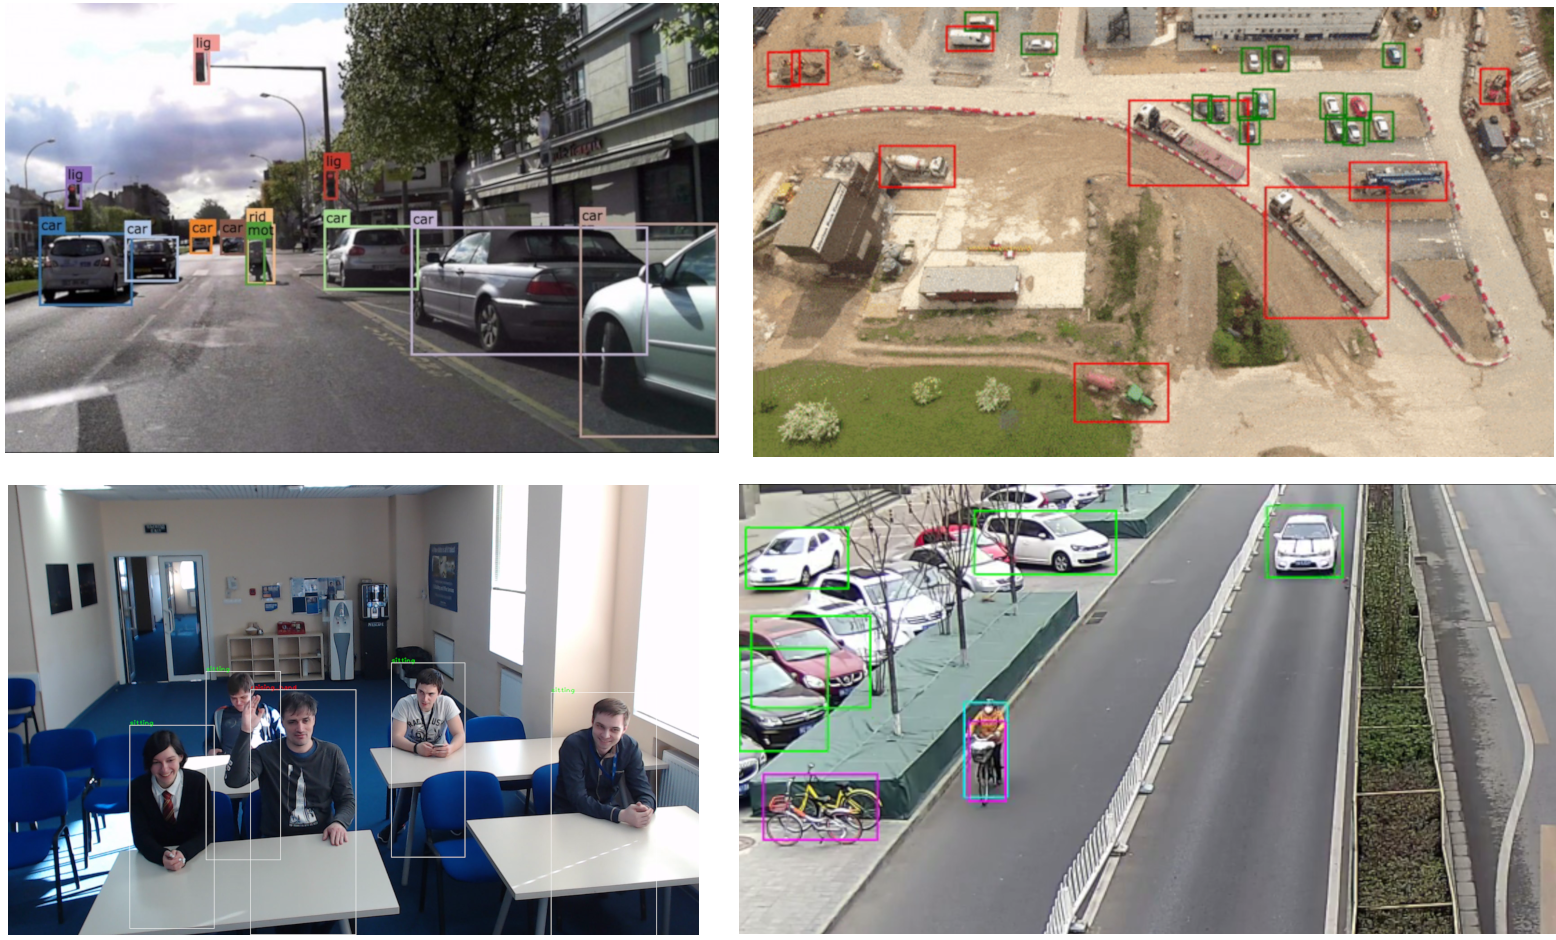
\includegraphics[scale=0.5]{1m.png} 
     	%\vspace*{-0.5em}
		%\caption{Floating gate transistor cell}
	\end{figure}
				
    \end{frame}
    
    \subsection{On top of that:}
	    
	\begin{frame}
	
	Object detection can have other constraints:	
	\vspace*{1em}	
	
	\begin{itemize}
		\item{\textbf{real-time} detection}
		\item{work on \textbf{embedded systems}
		\begin{itemize}
			\item{ex: cars, UAVs, etc.}
		\end{itemize}				
		}
		\item{\textbf{weather conditions}}
		\item{\textbf{night conditions}}
		\item{etc.}
	\end{itemize}
	
	\begin{figure}
		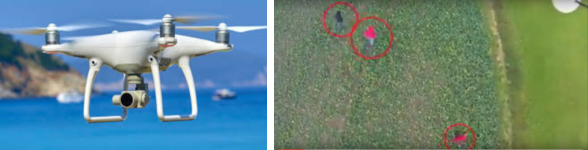
\includegraphics[scale=0.9]{2m.png} 
     	%\vspace*{-0.5em}
		%\caption{Floating gate transistor cell}
	\end{figure}

    \end{frame}	    
	    
	\subsection{Some applications}	
	    
	\begin{frame}
	
	Applications:
	\vspace*{1em}
	
	\begin{itemize}
	\item{Advanced Driver Assistance System (ADAS)
	\begin{figure}
		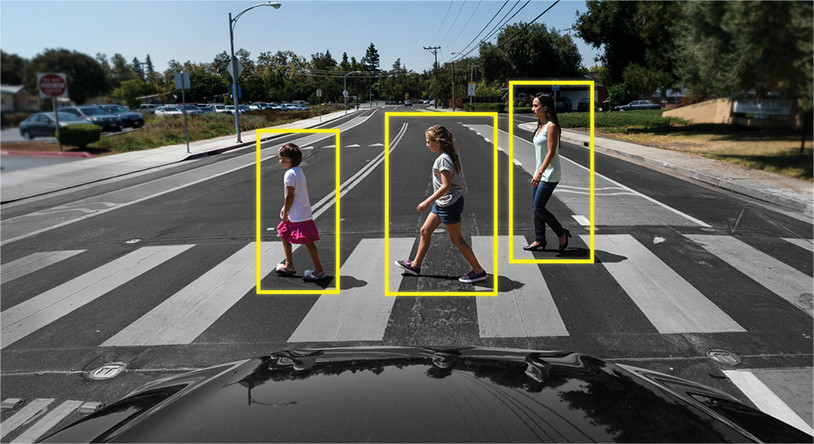
\includegraphics[scale=0.2]{21.jpg} 
     	%\vspace*{-0.5em}
		%\caption{Floating gate transistor cell}
	\end{figure}		}
	\item{Video surveillance:
	\begin{figure}
		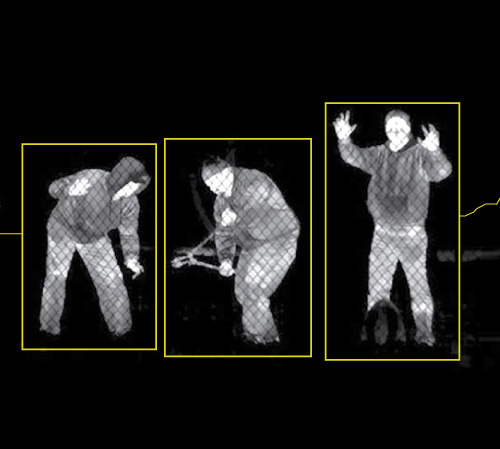
\includegraphics[scale=0.9]{22.jpg} 
     	%\vspace*{-0.5em}
		%\caption{Floating gate transistor cell}
	\end{figure}	}
	
	\end{itemize}
	
    \end{frame}	 
	
	\begin{frame}
	
	\begin{itemize}
	\item{Robots
	
	\begin{figure}
		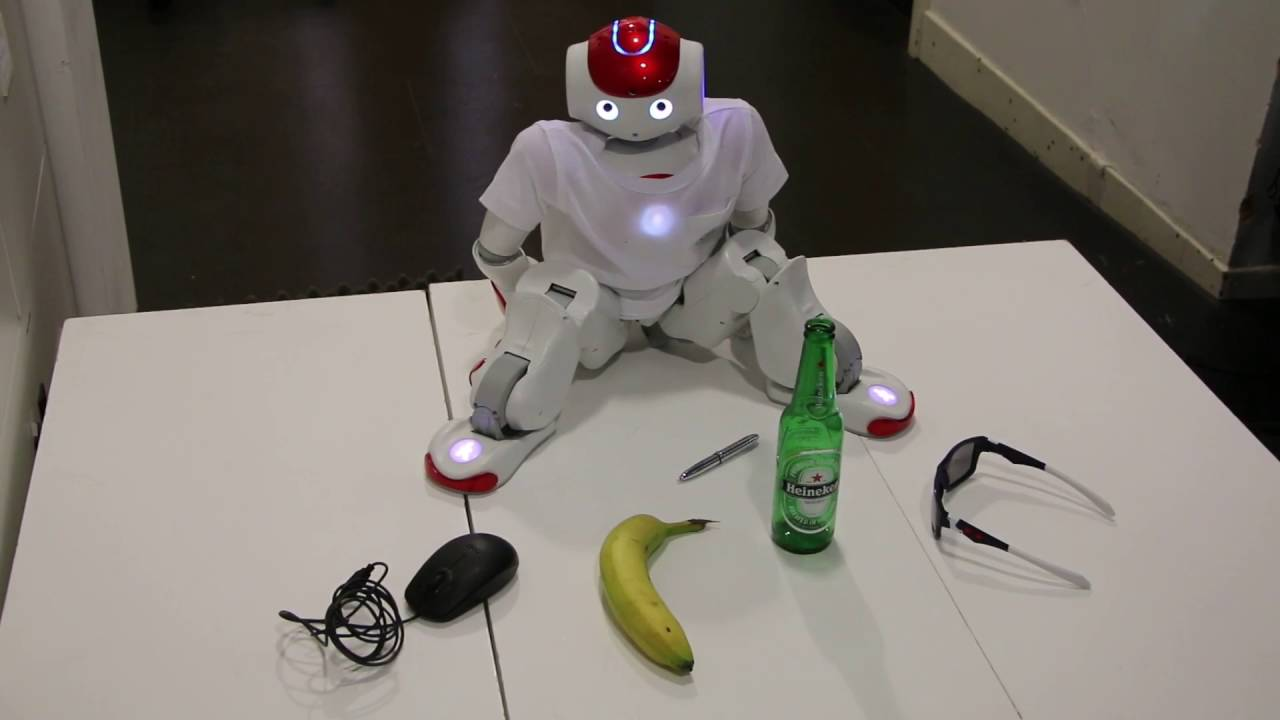
\includegraphics[scale=0.1]{23.jpg} 
     	%\vspace*{-0.5em}
		%\caption{Floating gate transistor cell}
	\end{figure}	
	
	}	
	\item{Face detection 
	
	\begin{figure}
		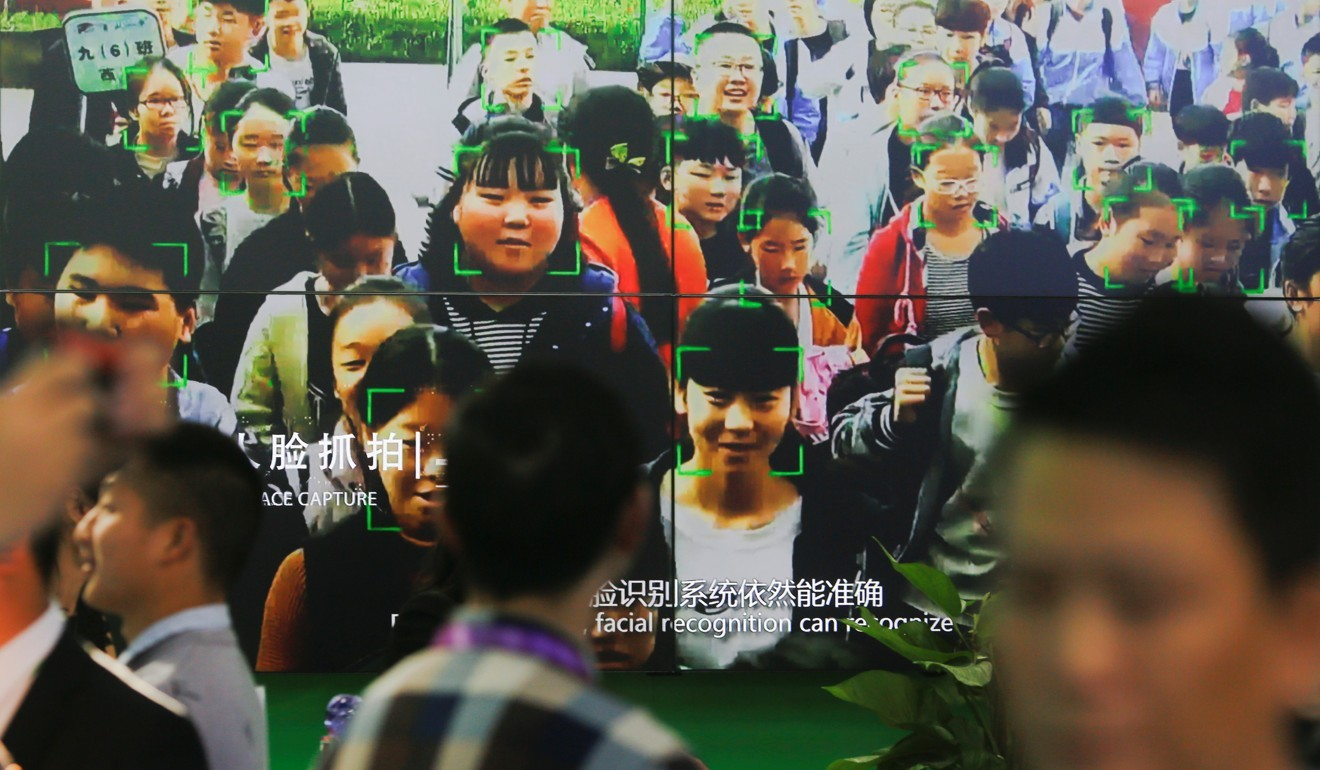
\includegraphics[scale=0.1]{24.jpg} 
     	%\vspace*{-0.5em}
		%\caption{Floating gate transistor cell}
	\end{figure}			
	}
%	\item{Face check (+recognition)
%	\begin{figure}
%		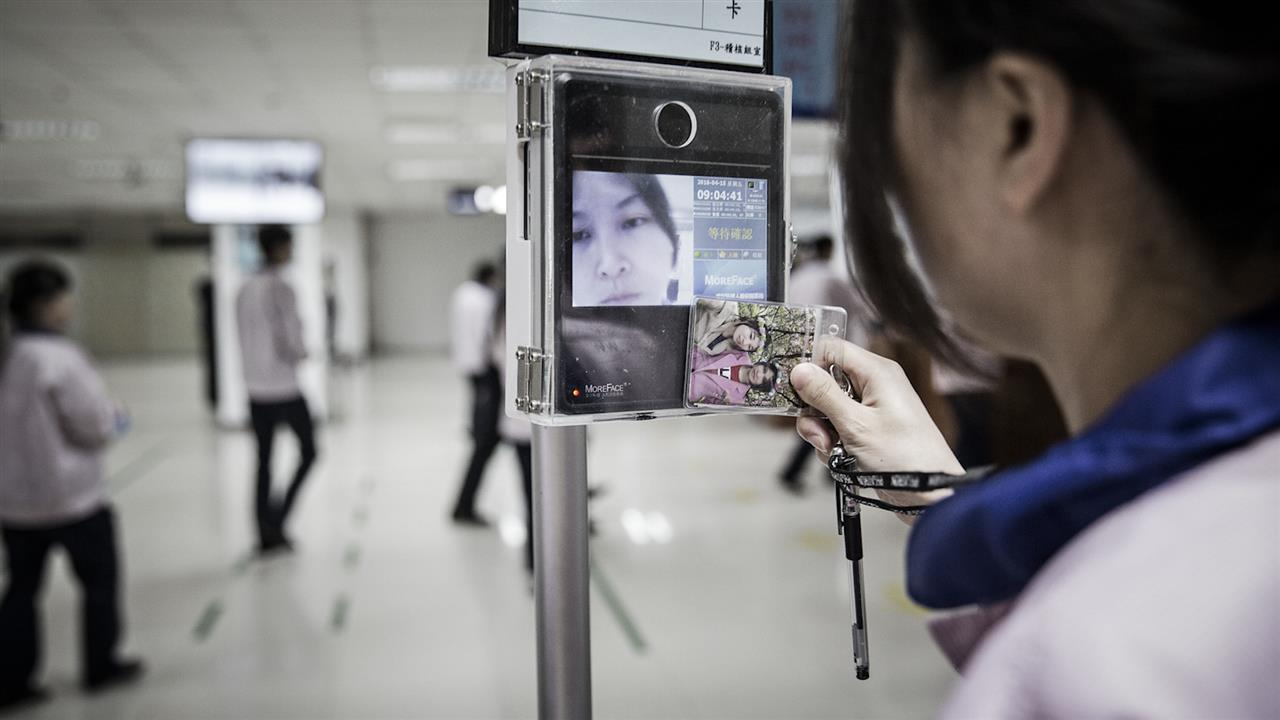
\includegraphics[scale=0.1]{25.jpg} 
%     	%\vspace*{-0.5em}
%		%\caption{Floating gate transistor cell}
%	\end{figure}	
%	}
	\item{...}
	
	\end{itemize}
	
	\end{frame}	
	
	    	        
	\section{How to detect objects in an image?}    
    \subsection{Example}
    \begin{frame}
    How to find these monkeys?
    \vspace*{1.0em}	
	
	\begin{figure}
		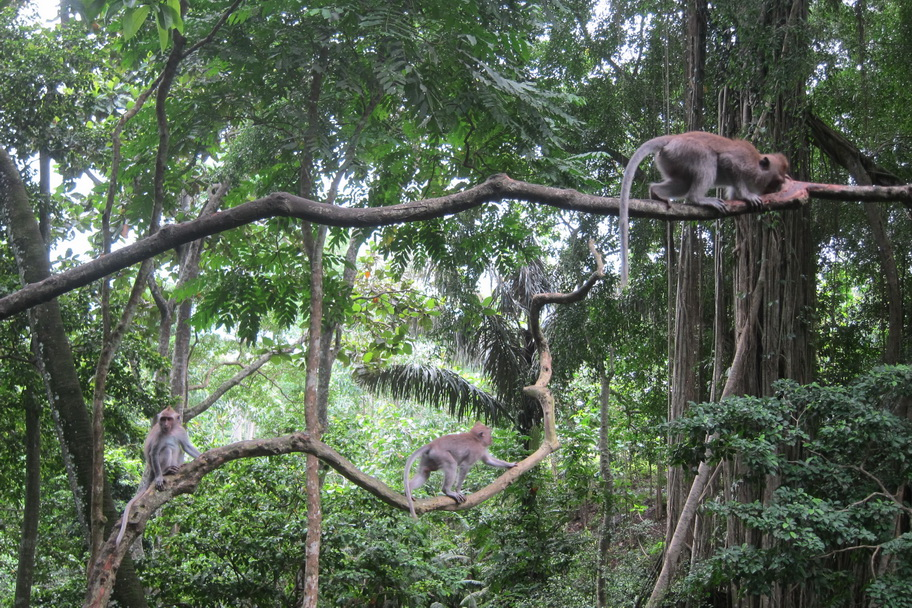
\includegraphics[scale=0.3]{monkey-1.jpg} 
     	%\vspace*{-0.5em}
		%\caption{Floating gate transistor cell}
	\end{figure}

   \end{frame}
    
    \subsection{Search at multiple locations}
    \begin{frame}

	Searching at multiple locations
	\vspace*{1.0em}	
	
\begin{columns}
\begin{column}{0.5\textwidth}
	\begin{figure}
		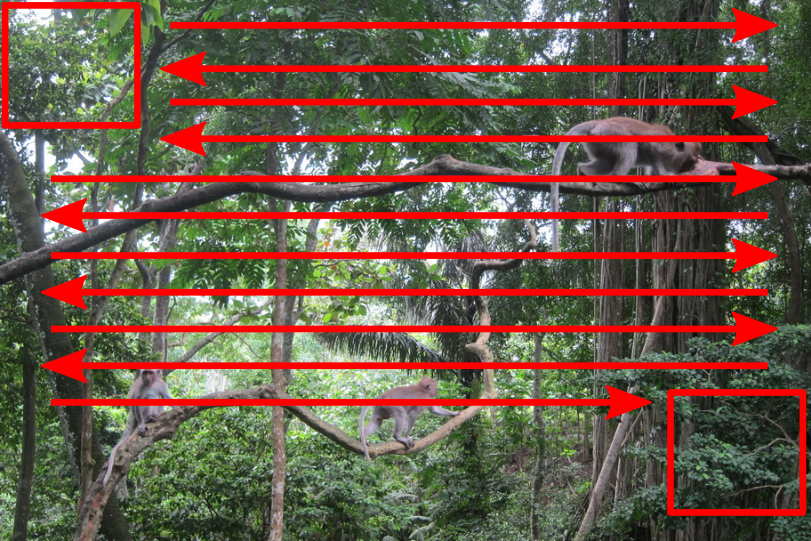
\includegraphics[scale=0.2]{monkey-2.jpg} 
     	%\vspace*{-0.5em}
		%\caption{Floating gate transistor cell}
	\end{figure}	 
\end{column}
\begin{column}{0.5\textwidth}  %%<--- here
    \begin{center}
	\begin{itemize}
	\item{\textbf{Sliding Window: \newline Exhaustive scan of the image}}
	\end{itemize}	     
     
     \end{center}
\end{column}
\end{columns}	
	

			
    \end{frame}

    \begin{frame}

	Searching at multiple locations
	\vspace*{1.0em}	
	
\begin{columns}
\begin{column}{0.5\textwidth}
	\begin{figure}
		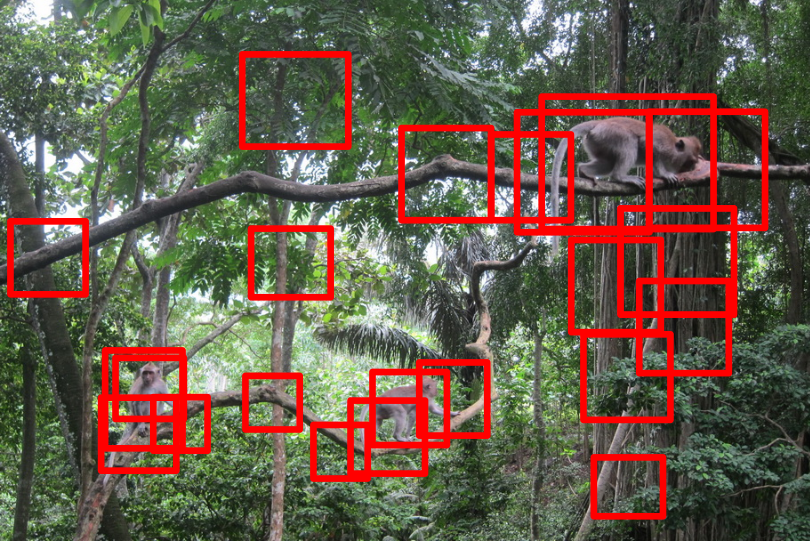
\includegraphics[scale=0.2]{monkey-3.jpg} 
     	%\vspace*{-0.5em}
		%\caption{Floating gate transistor cell}
	\end{figure}	 
\end{column}
\begin{column}{0.5\textwidth}  %%<--- here
    \begin{center}
	\begin{itemize}
	\item{Sliding Window: \newline Exhaustive scan of the image}
	\newline
	\item{\textbf{Generate region proposals: \newline Info-rich regions are proposed}}
	\end{itemize}	     
     
     \end{center}
\end{column}
\end{columns}		
	
	
	
	\end{frame}
	
	 \subsection{Search at multiple scales}
    \begin{frame}

	Searching at multiple scales
	\vspace*{1.0em}	
	
\begin{columns}
\begin{column}{0.5\textwidth}
	\begin{figure}
		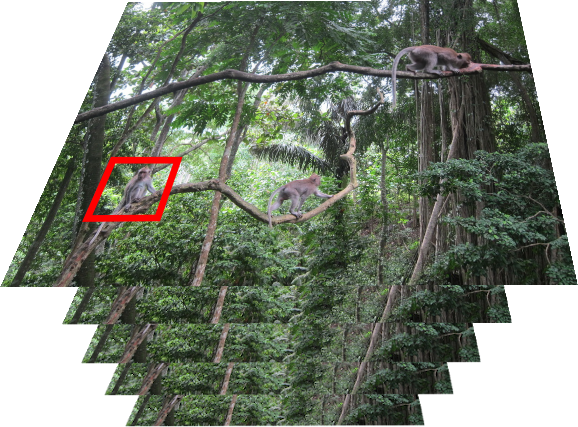
\includegraphics[scale=0.3]{monkey-4.png} 
     	%\vspace*{-0.5em}
		%\caption{Floating gate transistor cell}
	\end{figure}	 
\end{column}
\begin{column}{0.5\textwidth}  %%<--- here
    \begin{center}
	\begin{itemize}
	\item{Analysis window 
		\begin{itemize}
			\item{Fixed size}
		\end{itemize}			
	}
	\item{Image pyramid
		\begin{itemize}
		\item{Down-scaled levels for big objects}
		\item{Up-scaled levels for small objects}
		\end{itemize}			
	}
	\end{itemize}	     
     
     \end{center}
	\end{column}
	\end{columns}	
				
    \end{frame}
	
	\subsection{Finding clues}
    \begin{frame}

	Finding clues
	\vspace*{1.0em}	
	
\begin{columns}
\begin{column}{0.5\textwidth}
	\begin{figure}
		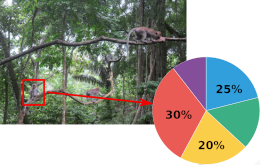
\includegraphics[scale=0.6]{monkey-5.png} 
     	%\vspace*{-0.5em}
		%\caption{Floating gate transistor cell}
	\end{figure}	 
\end{column}
\begin{column}{0.5\textwidth}  %%<--- here
    \begin{center}
	\begin{itemize}
	\item{Visual features
		\begin{itemize}
		\item{\textbf{Colors}}
		\end{itemize}			
	}
	\end{itemize}	     
     
     \end{center}
	\end{column}
	\end{columns}	
				
    \end{frame}
	
    \begin{frame}

	Finding clues
	\vspace*{1.0em}	
	
\begin{columns}
\begin{column}{0.5\textwidth}
	\begin{figure}
		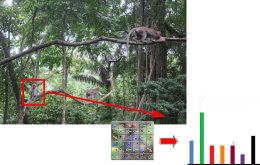
\includegraphics[scale=0.6]{monkey-6.png} 
     	%\vspace*{-0.5em}
		%\caption{Floating gate transistor cell}
	\end{figure}	 
\end{column}
\begin{column}{0.5\textwidth}  %%<--- here
    \begin{center}
	\begin{itemize}
	\item{Visual features
		\begin{itemize}
		\item{Colors}
		\item{\textbf{Shapes}}
		\end{itemize}			
	}
	\end{itemize}	     
     
     \end{center}
	\end{column}
	\end{columns}	
				
    \end{frame}	
	
	\begin{frame}

	Finding clues
	\vspace*{1.0em}	
	
\begin{columns}
\begin{column}{0.5\textwidth}
	\begin{figure}
		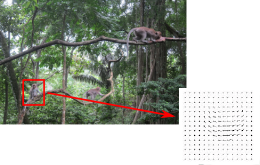
\includegraphics[scale=0.6]{monkey-7.png} 
     	%\vspace*{-0.5em}
		%\caption{Floating gate transistor cell}
	\end{figure}	 
\end{column}
\begin{column}{0.5\textwidth}  %%<--- here
    \begin{center}
	\begin{itemize}
	\item{Visual features
		\begin{itemize}
		\item{Colors}
		\item{Shapes}
		\item{\textbf{Movements}}
		\item{\textbf{Etc.}}
		\end{itemize}			
	}
	\end{itemize}	     
     
     \end{center}
	\end{column}
	\end{columns}	
				
    \end{frame}
	
		
 \subsection{Analyze the collected clues and decide!}
    \begin{frame}

	Analyze the collected clues and decide!
	\vspace*{1.0em}	
	
\begin{columns}
\begin{column}{0.5\textwidth}
	\begin{figure}
		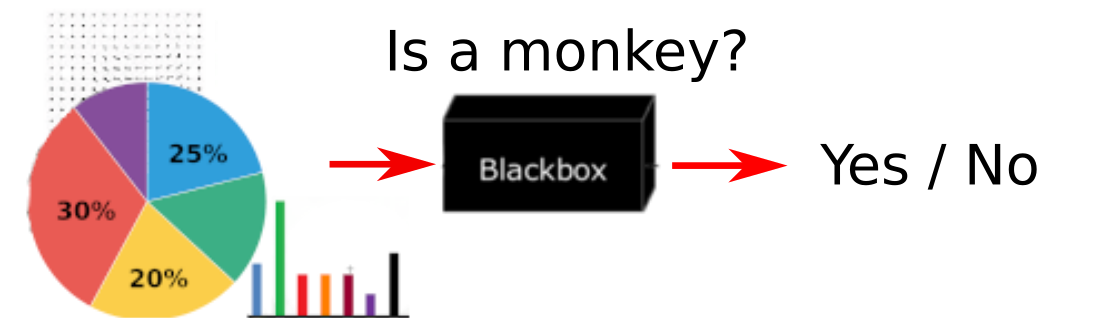
\includegraphics[scale=0.15]{monkey-8.png} 
     	%\vspace*{-0.5em}
		%\caption{Floating gate transistor cell}
	\end{figure}	 
\end{column}
\begin{column}{0.5\textwidth}  %%<--- here
    \begin{center}
	\begin{itemize}
	\item{Classify
		\begin{itemize}
			\item{Visual features of a monkey...}
			\item{...or not\newline}
			
		\end{itemize}			
	}

	\item{Deep learning
		\begin{itemize}
		\item{All these steps may be combined}
		\end{itemize}			
	}
	\end{itemize}	     
     
     \end{center}
	\end{column}
	\end{columns}	
				
    \end{frame}		
		
		
	\section{Training the blackbox with Machine Learning}    
    
	\subsection{Joining Computer Vision and Machine Learning}    
    
    \begin{frame}
	

	How to train the blackbox (classifier)? With Machine Learning!		
	\vspace*{0.5em}
	
	\begin{itemize}	
	\item{Papageorgiou et al: Training the classifier with a SVM algorithm}
	\end{itemize}

	\begin{figure}
		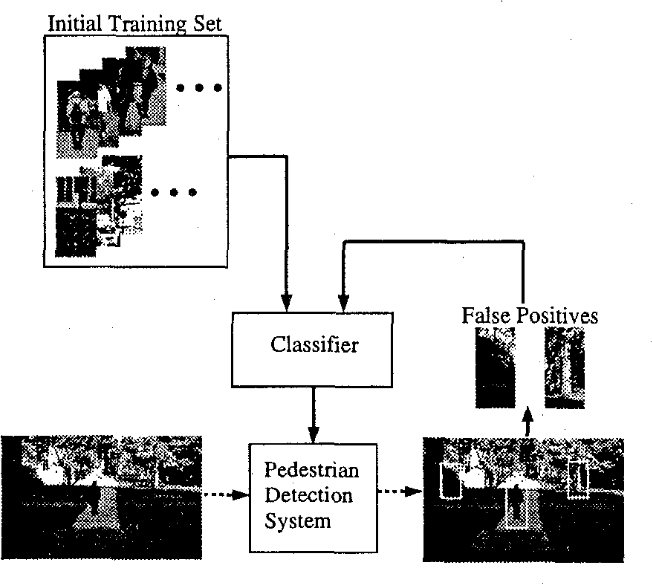
\includegraphics[scale=0.5]{27.png} 
     	%\vspace*{-0.5em}
		%\caption{Floating gate transistor cell}
	\end{figure}
	
    \end{frame}    
    
    \subsection{Learning models 1}    
    
    \begin{frame}
	
	At first, to \textbf{train the blackbox} we \textbf{need a lot of image examples}:
	\vspace*{1em}	
	
	\begin{itemize}
	\item{images of \textbf{object} (ex: images of people)}
	\item{images of \textbf{random background}}	
	\end{itemize}	 
	\vspace*{0.5em}	
	
	\begin{figure}
		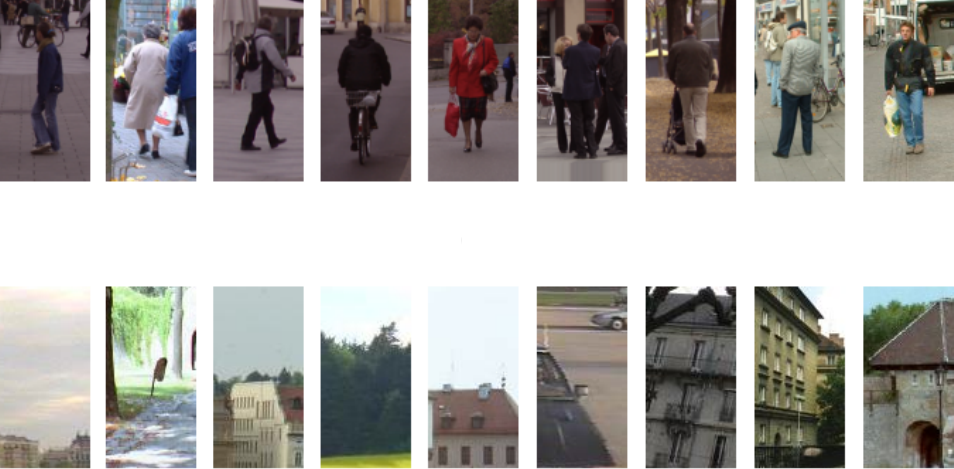
\includegraphics[scale=0.5]{18.png} 
     	%\vspace*{-0.5em}
		%\caption{Floating gate transistor cell}
	\end{figure}
	
	\end{frame}    
    
   \subsection{Learning models 2}    
    
    \begin{frame}
	
	Then, we can \textbf{train the blackbox} with a Machine Learning algorithm:
	\vspace*{1em}
	\begin{itemize}
	\item{Support Vector Machine (SVM)
	\begin{figure}
		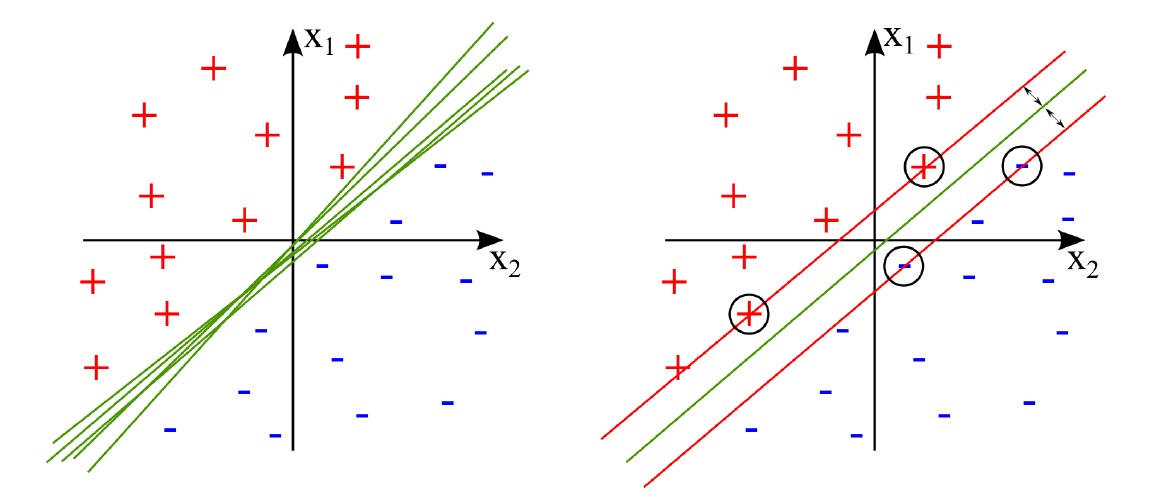
\includegraphics[scale=0.28]{19.png} 
     	%\vspace*{-0.5em}
		%\caption{Floating gate transistor cell}
	\end{figure}
	
	}
	\item{Boosting 
	\begin{figure}
		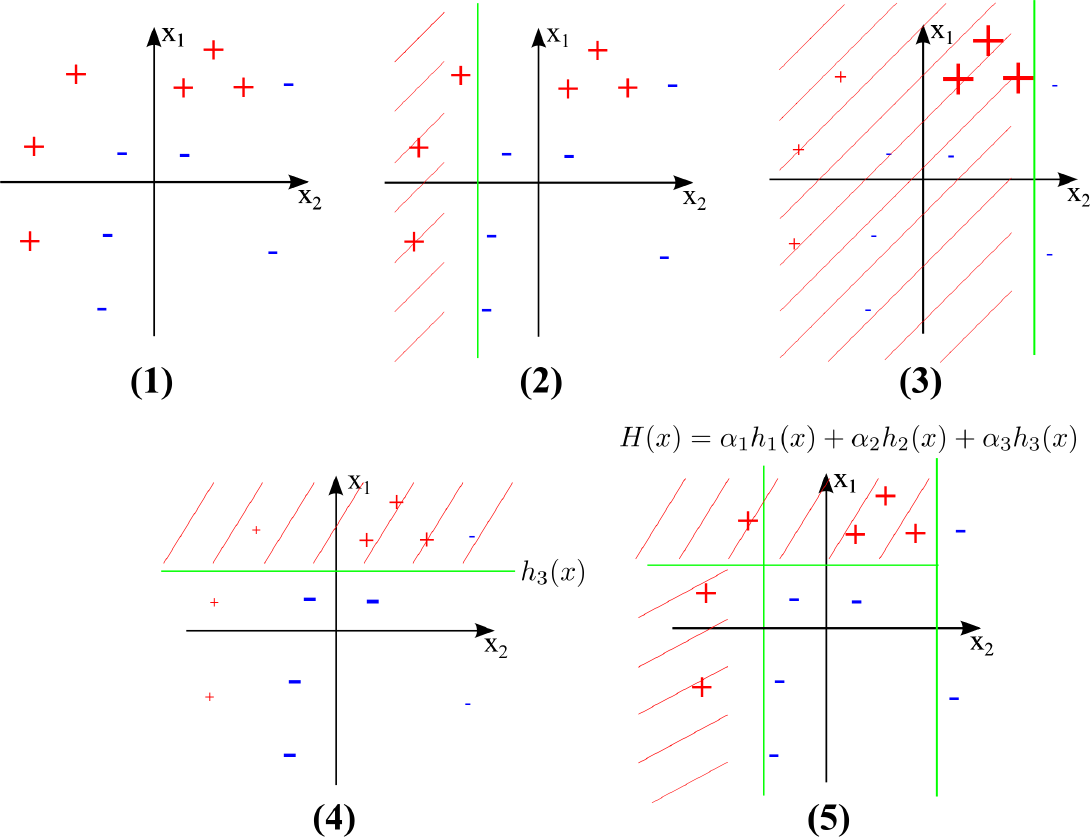
\includegraphics[scale=0.35]{20.png} 
     	%\vspace*{-0.5em}
		%\caption{Floating gate transistor cell}
	\end{figure}
	
	}
	\end{itemize}		
	
	\end{frame} 
        
	\subsection{Reaching the ceiling of model improvements}    
    
    \begin{frame}
	
	Before ~2014, there have been some \textbf{improvements}:
	\vspace*{1em}
	
	\begin{itemize}
	\item{New classifiers (Soft-Cascade Boosting, Latent-SVM, etc))
	\begin{columns}
\begin{column}{0.5\textwidth}
	 \begin{figure}
		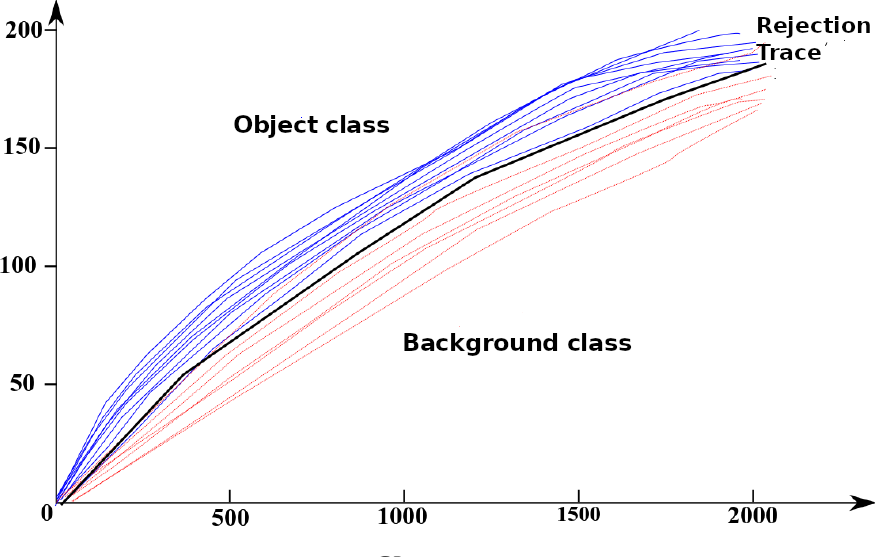
\includegraphics[scale=0.20]{21.png} 
     	%\vspace*{-0.5em}
		%\caption{Floating gate transistor cell}
	\end{figure}	
\end{column}
\begin{column}{0.5\textwidth}  %%<--- here
    \begin{center}
     	\begin{figure}
		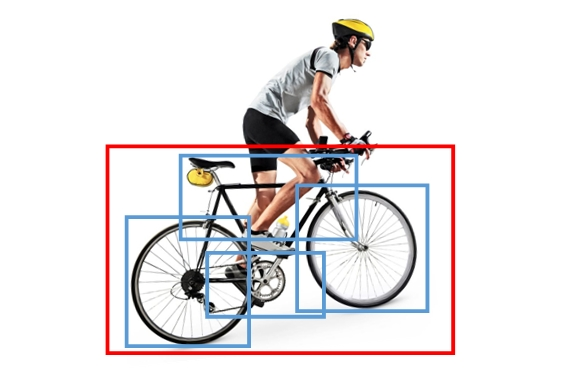
\includegraphics[scale=0.20]{20e.jpg} 
     	%\vspace*{-0.5em}
		%\caption{Floating gate transistor cell}
	\end{figure}
     
     \end{center}
	\end{column}
	\end{columns}
	
	}
	\item{New ways of collecting clues/features (HOG, ICF, ACF, etc)}
	\vspace*{1em}
	
	\end{itemize}	
	
	\begin{block}{With this approach ...}
	\textbf{NO real dramatic improvements... after 2014: Deep learning!} 
	\end{block}	
	
	\end{frame}  
    	
    \section{Deep learning}    

	\subsection{The come back of Neural Networks}    
    \begin{frame}
	
	The \textbf{COME BACK of Artificial Neural Networks}:
	\vspace*{1em}
	
	\begin{itemize}
		\item{Artificial Neural Networks (ANN) \textbf{exist for a very long time} (50's)}	
		\item{But: the more recent SVM beat ANNs for a while}
		\item{Among all ANN: \textbf{CNN} is the \textbf{most suitable for Computer Vision}}
		\item{Deep learning: deep means a network with more than 4/5 layers}
	\end{itemize}		
	\vspace*{1em}	
	
	The emergence of Deep learning is due to: 
	\vspace*{1em}

	\begin{itemize}
	\item{New network \textbf{learning approaches}}	
	\item{\textbf{Fixing some problems} (vanishing gradient, etc.)}
	\item{\textbf{More data} available everywhere}
	\item{More and more \textbf{powerful computers}}
	\end{itemize}
		

    \end{frame}    
    
   
	\subsection{CNN: The Convolutional Neural Network architecture}    
    \begin{frame}
	
	The Convolutional Neural Network (CNN) is as follow:
	\vspace*{1em}
	\begin{figure}
		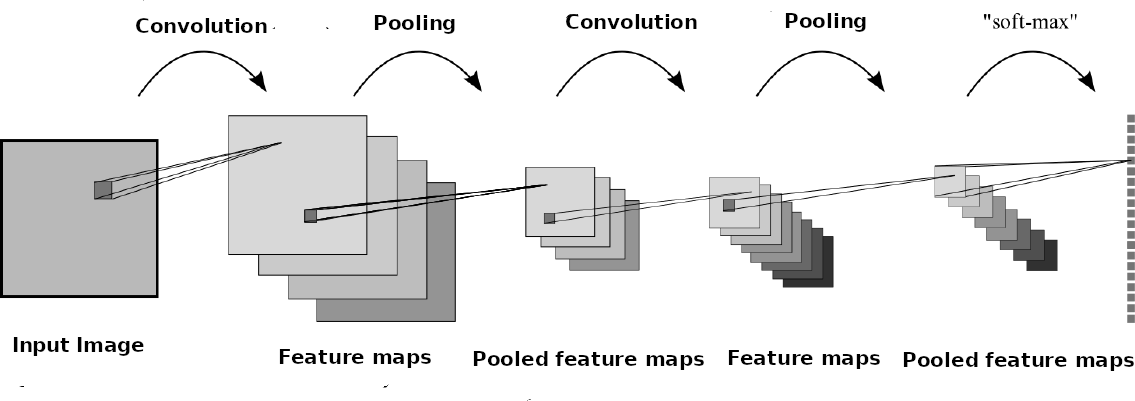
\includegraphics[scale=0.6]{30.png} 
     	%\vspace*{-0.5em}
		%\caption{Floating gate transistor cell}
	\end{figure}
	\vspace*{1em}
	
	\begin{itemize}
	\item{Convolution: \textbf{local pixels} are \textbf{connected to the same pool node}}
	\item{Pooling: \textbf{features} computed in the convolution layers \textbf{are aggregated} (max or average over a pool)}
	\item{Images = many pixels, thanks to CNN: we \textbf{don't need a tremendeous number of connections}}
	\end{itemize}

    \end{frame}   
    
    \subsection{The ImageNet DCNN revolution}    
    \begin{frame}

	In 2012 the first Deep CNN:
	\vspace*{1em}
	
	\begin{itemize}
	\item{It won the "ImageNet" contest (1.6 millions images):
		\begin{itemize}
			\item{Can reconize 1000 object types}
			\item{37.5\% error rate (previous best: 45.1\%)}
		\end{itemize}
	}
	
	\end{itemize}
	
	\begin{figure}
		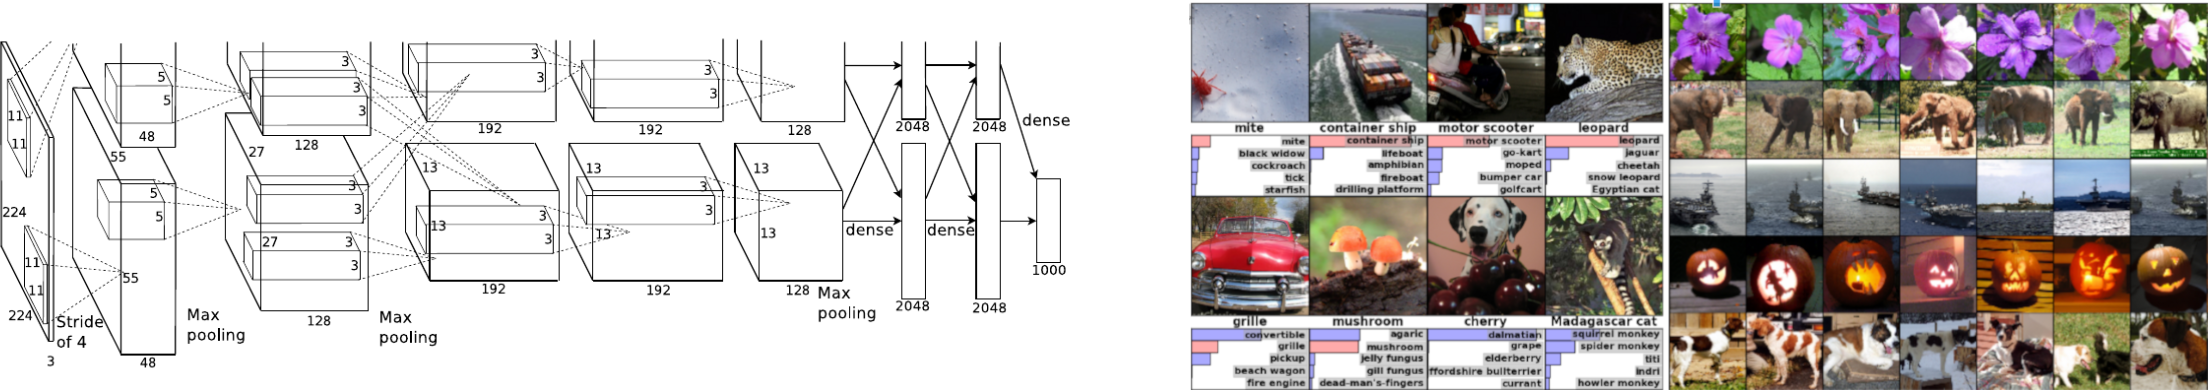
\includegraphics[scale=0.45]{31.png} 
     	%\vspace*{-0.5em}
		%\caption{Floating gate transistor cell}
	\end{figure}
	

	\vspace*{1em}
	
	\begin{block}{BUT:}
	It's NOT OBJECT DETECTION it's OBJECT CLASSIFICATION
	\end{block}
	 	
	\end{frame} 
	    
	\subsection{From classification to detection!}    
    \begin{frame}
		
	A series of improvements:
	\vspace*{1em}		
		
	\begin{itemize}
	\item{
	In 2014, R-CNN: it can detect objects!
	\begin{itemize}
		\item{Generate \textbf{region proposals} to search objects (Selective Search)}			
		\item{Use Deep CNN to collect clues/features}
		\item{53.7\% of mAP PASCAL 2010 (previous best: 33.4\%)\newline}
	\end{itemize}

	
	
	}
	\item{	
	In 2015, Fast R-CNN: faster
	\begin{itemize}
		\item{\textbf{All clues/features are computed once!}\newline}
	\end{itemize}	
	\begin{figure}
				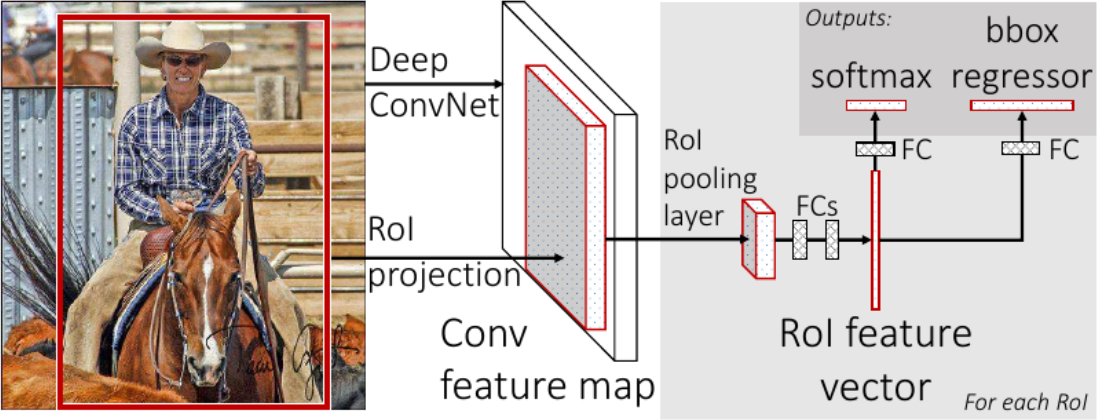
\includegraphics[scale=0.3]{32.png} 
					     	%\vspace*{-0.5em}
							%\caption{Floating gate transistor cell}
			\end{figure}	
		    
    }
    \item{
    The same year, Faster R-CNN: even faster
	\begin{itemize}
		\item{The network itself \textbf{generate region proposals}!\newline}
	\end{itemize}
	}
	\end{itemize}

	\end{frame} 	    
	    
	   	      
	\subsection{Residual learning: even bigger networks}    
    \begin{frame}

	So far, "deep" meant 4/5 layers, but \textbf{residual learning} permits more:

	\vspace*{2em}
	
	\begin{itemize}
		\item{This is a "residual mapping" ($F(x) + X$)
			\begin{figure}
				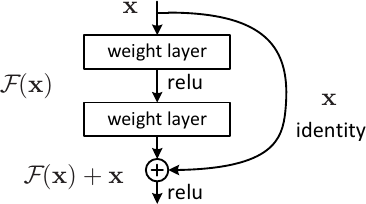
\includegraphics[scale=0.5]{34.png} 
					     	%\vspace*{-0.5em}
							%\caption{Floating gate transistor cell}
			\end{figure}				
		}
		\item{The architecture of the network can have >100 layers with this!}
		\item{19.38\% error rate on ImageNet! (previous best: 37.5\%)}
	\end{itemize}
	\vspace*{2em}	
	
	\textbf{Residual learning means better detection performance!}

    \end{frame}      
    
    \begin{frame}
    
    	\begin{figure}
			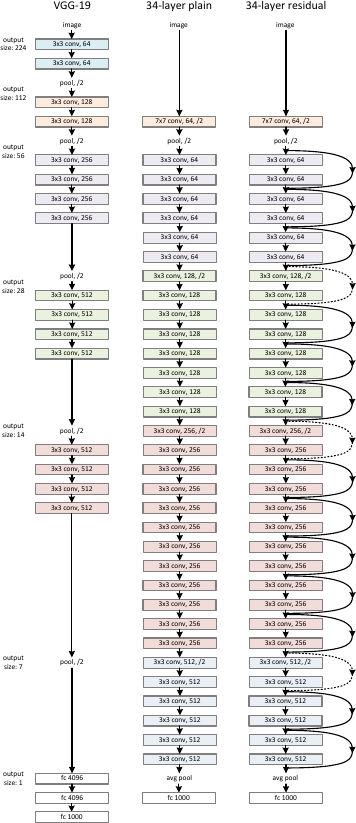
\includegraphics[scale=0.7]{35.png} 
					     	%\vspace*{-0.5em}
							%\caption{Floating gate transistor cell}
		\end{figure}
    
    \end{frame}
	    
    
	\subsection{Feature pyramid networks for multiscale}    
    \begin{frame}
    
	In 2017, FPN: more robust to object sizes!
	
	\vspace*{1em}    
    
	\begin{itemize}
		\item{There is an \textbf{image pyramid} \textbf{INSIDE the network}
			\begin{figure}
				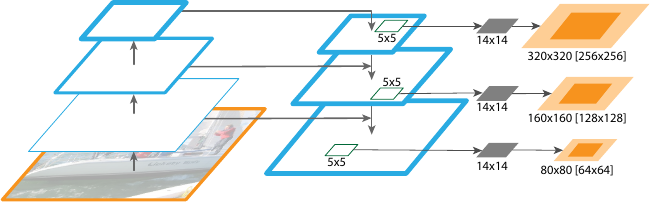
\includegraphics[scale=0.7]{36.png} 
			\end{figure}
		}
		\item{Faster R-CNN VS FPN: Improve by 2\% in AP (COCO dataset)}
	
	\end{itemize}	    
	\vspace*{1em}    	 	
    	
    \begin{block}{Detection performance} 	
	\textbf{Accuracy gets improved again!}    	 
	\end{block}	
    	 	
    \end{frame}	    
	        
    \subsection{Alternative: the regression approach}    
    \begin{frame}

	In 2016, YOLO: an alternative approach

	\vspace*{1em}	
	
	\begin{itemize}
		\item{Here: it is a \textbf{regression problem}
			\begin{itemize}
				\item{all combined: \textbf{search}, \textbf{extract clues/features} AND \textbf{infer}}			
				\item{so, there is \textbf{no need to generate region proposals}}
						
			\end{itemize}	}	
			\item{Learn the context as well (more general)}		
			\item{More \textbf{easy to train}}
			\item{Much faster: 45 FPS on Titan GPU!}
		\end{itemize}							
			
		
			
			\begin{figure}
						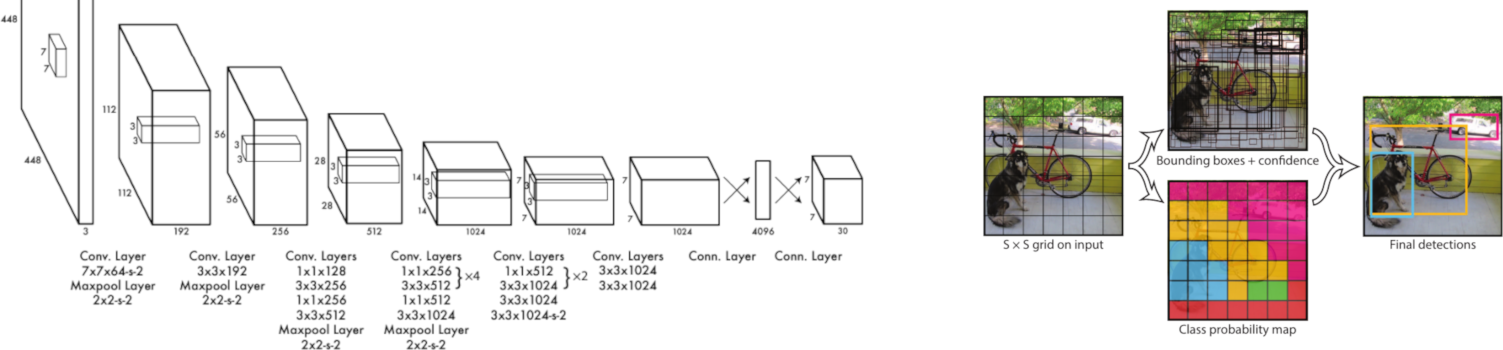
\includegraphics[scale=0.5]{37.png} 
					     	%\vspace*{-0.5em}
							%\caption{Floating gate transistor cell}
			\end{figure}	
	
    \end{frame}  
    
    \subsection{RetinaNet: Reaching classification performance!}    
    \begin{frame}

	In 2017, RetinaNet: Regression outperformed classification!	
	
	\vspace*{0.5em}
	
	\begin{itemize}
		\item{A new training loss function to optimize:
			\begin{itemize}
				\item{Called Focal Loss}
				\item{\textbf{Focus} the learning on \textbf{hard background images}}
			\end{itemize}					
		}	
		\item{Outperforms all classification approaches on COCO (speed VS AP)!
			\begin{figure}
				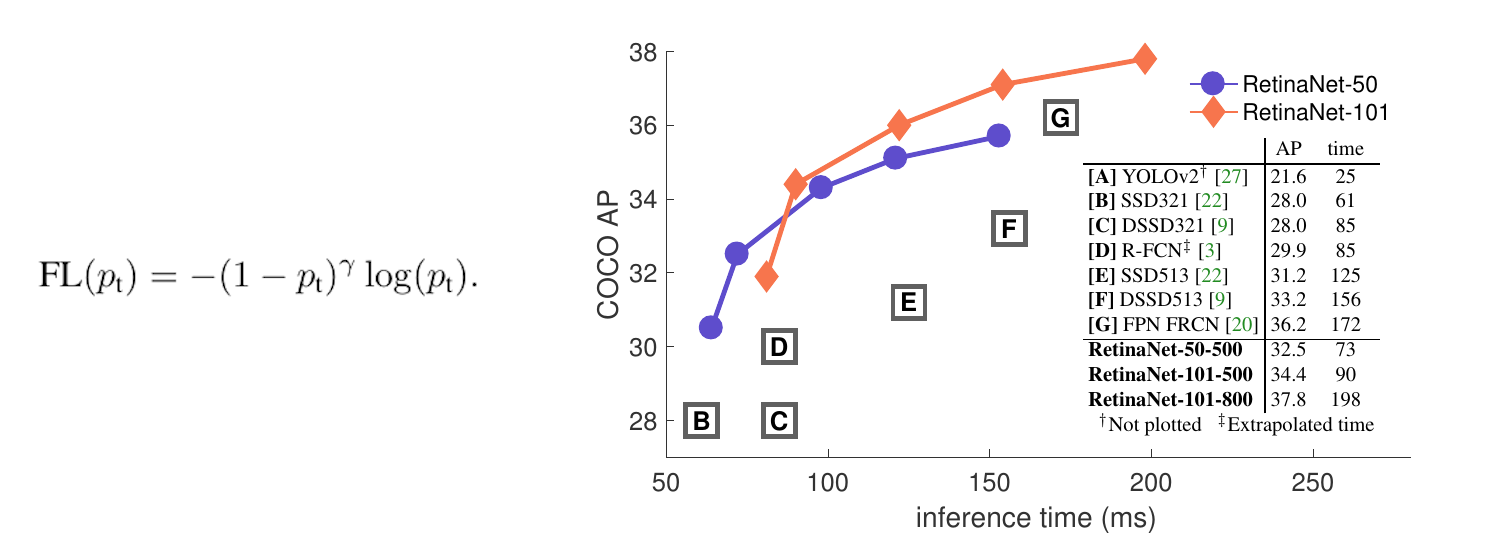
\includegraphics[scale=0.45]{39.png} 
				%\vspace*{-0.5em}
				%\caption{Floating gate transistor cell}
				\end{figure}		
		}
		
	\end{itemize}		
	\vspace*{0.5em}
	
	\textbf{A great step towards a all-in-one network object detector}	
	
    \end{frame} 
    
    \section{Conclusion}   
    
	  
    
     \begin{frame}
     
     To conclude:
		\vspace*{1em}  
     
		\begin{itemize}
			
			\item{Former Machine Learning approaches for OD: obsolete}    
		 	\item{Performances improved thanks to Deep Learning}
			\item{Year after year, Deep Learning-based Object Detection becomes ...
				\begin{itemize}
					\item{... simpler (one step training, etc.)}		
					\item{... more accessible (cheaper and cheaper powerful GPU, etc.)}
					\item{... more accurate (new optimizations, etc.)} 
					\item{... speeder.}
				\end{itemize}}
			\item{A clear trend: one unique network for all detection steps}
		\end{itemize}
		\vspace*{1em}

		In 2018, YOLOv3: two to three times faster than RetinaNet, with same accuracy ... 
		\vspace*{1em}

		\textbf{The course continue...}
		
	\end{frame}  
    
	    
    
	
\end{document}
